\begin{figure}[!htb]
    \begin{center}
    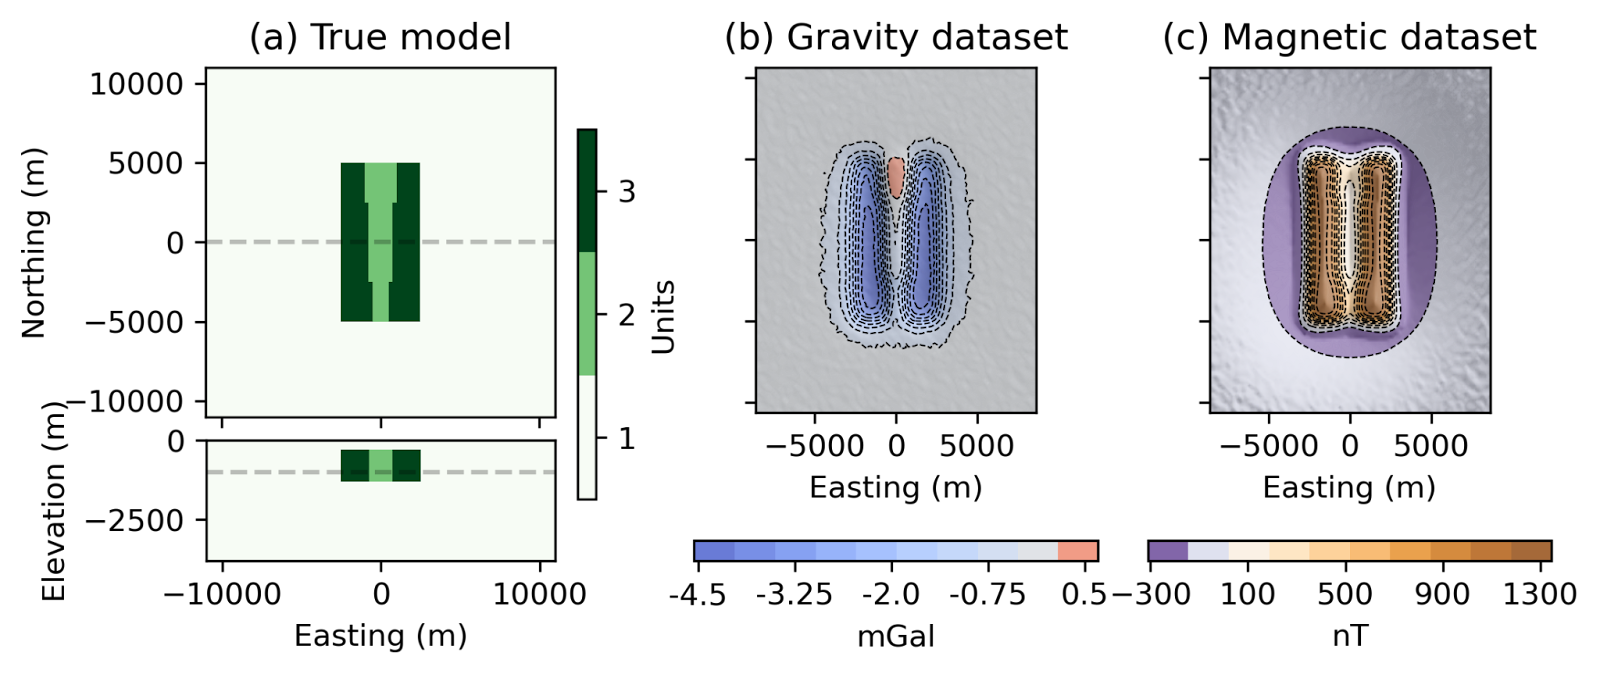
\includegraphics[width=0.95\textwidth]{figures/joint-inversion-setup.png}
    \end{center}
\caption{
    (a) Synthetic model for the carbon mineralization example. The serpentinized unit, unit 3, has a density of 2.7 g/cc,  and 0.15 SI susceptibility.  The carbonated unit, unit 2, has a density of 3.0 g/cc and 0.05 SI susceptibility. The background, unit 1, has a density of 2.9 g/cc and 0 susceptibility. (b) Gravity (c) and magnetic data are simulated on a 19 km by 21 km grid with 250 m grid spacing. After \citep{capriotti_joint_2023}.
}
\label{fig:joint-inversion-setup}
\end{figure}
